\section{Datenbankzugriff}\label{sec:datenbankzugriff}
Die zentrale Komponente unseres Systems ist die Datenbank. In sie fügt der Crawler neue Datensätze ein und aktualisiert vorhandene. Der Kategorisierer ist dafür zuständig die gefundenen Accounts nach der DMOZ.org Datenbank in Kategorien zu unterteilen. Die GUI wiederum ist die Komponente die die Daten aus der Datenbank ausliest und visualisiert. Gegebenenfalls kann sie auch Einträge hinzufügen, verändern beziehungsweise vervollständigen.
\\Da alle unsere drei Systemkomponenten lesend, sowie schreibend auf die Datenbank zugreifen, haben wir uns entschlossen ein Paket für den Datenbankzugriff für alle Komponenten zur Verfügung stellen. Dieses sogenannte mysql-Package ist dann für den Auf- und Abbau der Verbindung zur Datenbank zuständig, sowie für das Schreiben und Lesen in beziehungsweise aus der Datenbank. Es stellt für jede der drei Komponenten ein eigenes Interface zur Verfügung, sodass jede Komponente nur die für sie erlaubten Änderungen an der Datenbank vornehmen kann.
In \cref{fig:mysql-package} ist der Aufbau des mysql-Packages zu sehen. Das darin eingeschlossene result-Package stellt Objekt und Methoden zu Verfügung um die Ergebnisse aus der Datenbank zu speichern und zu verarbeiten.\\

\begin{figure}[h!]
	\centering
	\includegraphics[width=\textwidth,height=\textheight,keepaspectratio=true]{dia/uml_mysql-package}
	\caption{UML-Klassendiagramm des mysql-Packages}
	\label{fig:mysql-package}
\end{figure}

\begin{description}
	\item[AccessData] Klasse zur Verwaltung von Zugriffsdaten für die Datenbank.
	\item[DBConnection] Abstrakte Klasse die eine Verbindung zu einer Datenbank aufbaut und diese Verbindung auch wieder trennt.
	\item[DBIcrawler] Interface, welches die Methoden spezifizieren die der Crawler für den Datenbankzugriff benötigt.
	\item[DBIcategorizer] Interface, welches die Methoden spezifizieren die der Kategorisierer für den Datenbankzugriff benötigt.
	\item[DBIgui] Interface, welches die Methoden spezifizieren die die GUI für den Datenbankzugriff benötigt.
	\item[DBcrawler] Diese Klasse implementiert die Methoden des DBIcrawler Interfaces und stellt dem Crawler eine Datenbankverbindung zur Verfügung.
	\item[DBcategorizer] Diese Klasse implementiert die Methoden des DBIcategorizer Interfaces und stellt dem Kategorisierer eine Datenbankverbindung zur Verfügung.
	\item[DBgui] Diese Klasse implementiert die Methoden des DBIgui Interfaces und stellt dem der GUI eine Datenbankverbindung zur Verfügung.
	\item[Index] Als abstrakte Klasse stellt Index eine Möglichkeit zum Speichern des Datenbankindexes von Datenbankeinträgen zur Verfügung.
	\item[Account] In dieser Klasse werden einzelne Accounts verwaltet und gespeichert.
	\item[Retweets] In dieser Klasse werden nach Orten (und eventuell nach Daten) gruppierte Retweets verwaltet und gespeichert.
	\item[Tweets] In dieser Klasse werden nach Daten gruppierte Tweets verwaltet und gespeichert.
	\item[Location] In dieser Klasse werden einzelne Orte verwaltet und gespeichert.
	\item[Category] In dieser Klasse werden einzelne Kategorien verwaltet und gespeichert.
	\item[TweetsAndRetweets] Diese Klasse wird benutzt um zusammengefasste Daten der Datenbank an die GUI weiter zu leiten.
\end{description}

\section{ER-Modell}
Die Datenbank besteht aus sieben Tabellen, die über Fremdschlüssel miteinander in Relation stehen (s. \cref{fig:mysql-er}).\\

\begin{figure}[h!]
	\centering
	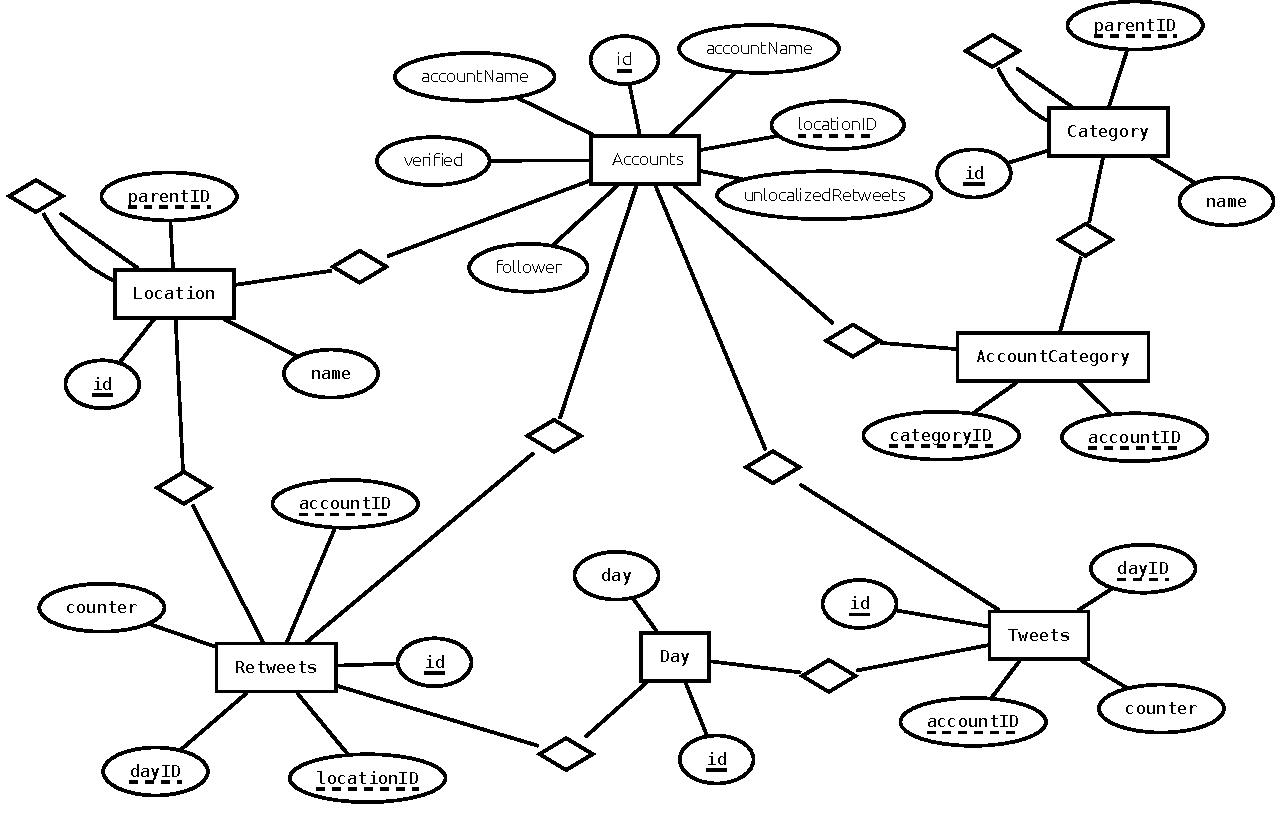
\includegraphics[width=\textwidth,height=\textheight, keepaspectratio=true]{dia/er}
	\caption{ER-Modell der MySQL-Datenbank}
	\label{fig:mysql-er}
\end{figure}

\begin{description}
	\item[accounts] Enthält alle verifizierten Accounts, die der Crawler im Twitter Stream mitgelesen hat, bzw. auch nicht verifizierte Accounts, die in der GUI hinzugefügt wurden. Dabei entspricht \emph{TwitterAccountId} der ID des Accounts in Twitter und \emph{id} ist ein Datenbank interner Primärschlüssel. Die Attribute \emph{Verified}, \emph{URL} und \emph{AccountName} entsprechen jeweils in Twitter hinterlegten Daten. \emph{Categorized} gibt an ob dieser Account bereits kategorisiert wurde und \emph{LocationId} Enthält den vom Loakaliserer berechneten zugehörigen Ort.
	\item[category] speichert die hierarchisch strukturierten (\emph{ParentId}) Kategorien.
	\item[page] In dieser Tabelle werden die einzelnen Webseiten (\emph{page}) gespeichert. Die Informationen dazu stammen aus der geparsten DMOZ-Datenbank.
	\item[accountCategory] Stellt die Relation zwischen	\emph{accounts} und \emph{category} in einer separaten Tabelle her, da einem Account mehrere Kategorien zugeordnet werden können.
	\item[location] Enthält die vom Lokalisierer ermittelten Orte, die jeweils \emph{Code} und \emph{Name} enthalten und auch per \emph{ParentId} hierarchisch gegliedert sein können.	
	\item[day] Enthält unterschiedliche Daten (\emph{Day}), die mittels \emph{Id} referenziert werden.
	\item[tweets] Beinhaltet die Anzahl der Tweets (\emph{Counter}) eines Accounts (\emph{AccountId}) an einem bestimmten Tag (\emph{DayId}).
	\item[retweets] Speichert die Anzahl der Retweets (\emph{Counter}) auf Tweets eines Accounts (\emph{AccountId}) an einem bestimmten Tag (\emph{DayID}) innerhalb eines bestimmten Lands bzw. Orts (\emph{LocationId}).
\end{description}

\section{Datenbankzugriff der GUI}
Da die GUI zur Visualisierung der Daten aus der Datenbank dient, ist es nötig, dass sie diese Daten in möglichst kompakter und vollständiger Form abrufen kann. Dazu stehen der GUI mehrere Möglichkeiten zur Verfügung die im Folgenden aufgelistet sind. Dabei sollen zum einen die Fähigkeiten der Datenbank ausgenutzt werden um Daten zusammenzufassen, zum Anderen sollen aber auch alle relevanten Daten einzeln zur Verfügung stehen.\\

\begin{description}
\item[Kategorien und Orte] Diese Informationen können jeweils als komplette Tabelle von der Datenbank geholt werden.
\item[Accounts] Mithilfe eines Account-Namens ist es möglich die AccountId herauszufinden. Außerdem können alle in der Datenbank vorhandenen Accounts geliefert werden. Dabei wird allerdings nur der Account-Name und die eigene Datenbank-Id übertragen.
\item[Tweets und Retweets] Um zu vorgegebenen Kategorien und Orten die Daten zu bekommen, sollen 4 Methoden zur Verfügung stehen. Im Folgenden werden jeweils nur die Tweets und Retweets von Accounts betrachtet, auf welche die Kategorie-Ort-Kombination/en passen.

\begin{itemize}
	\item Methoden, welche über alle Kalenderdaten summieren:
	\begin{itemize}
		\item Eine Methode liefert aggregierte Daten über die Summe der Tweets und Retweets pro Ort zurück, also für jeden Ort aus der Datenbank eine Summe von Tweets und eine Summe von Retweets.
		\item Eine weitere Methode liefert alle Accounts mit der Summe ihrer Tweets zurück auf die die Kategorie-Orts-Kombination passt. Dabei wird zu jeder Account-Orts Kombination eine Summe der Retweets mitgeliefert.
	\end{itemize}
	\item Methoden, welche die Daten nach Kalenderdaten separieren:
	\begin{itemize}
		\item Eine Methode liefert für jede Ort-Datums Kombination, die Summe über alle Tweets und Retweets zurück, sodass dann zu jedem Ort zu jedem Datum eine Summe von Tweets und Retweets bekannt ist.
		\item Eine weitere Methode liefert alle betroffenen Accounts zurück und pro Account noch die Anzahl der Retweets pro Ort pro Tag und die Tweets pro Tag.
	\end{itemize}
\end{itemize}
Die Berechnungen werden so weit möglich in die Datenbank ausgelagert, sodass diese die Summation übernimmt. Dadurch kann die Geschwindigkeit der Datenbank ausgenutzt werden und die Ressourcen auf Client-Seite werden geschont.
\end{description}

\section{Kategorisieren mit der DMOZ-Datenbank}
Zur Kategorisierung einzelner Accounts sollen die Informationen der DMOZ-Datenbank\footnote{Daten unter \url{http://www.dmoz.org/docs/en/rdf.html}} genutzt werden. Die Daten aus den zum Download angebotenen RDF-Dateien sollen in oben beschriebenes Tabellenlayout eingebettet werden. Hier soll kurz auf die Tags im RDF-Format eingegangen werden, sodass mit diesem Wissen ein Script zum Einlesen geschrieben werden kann.

\subsection{Einlesen der Kategorienhierarchie}\label{sec:katHierarchie}
Im Folgenden sind die relevanten Tags aufgelistet:
\begin{description}
	\item[topic] Das Attribut \lstinline{id} enthält den Kategorienamen im Format \emph{Top/World/Deutsch/...}. Aus diesem String soll der Baum erstellt werden.
	\item[narrow, narrow1, narrow2] Diese Tags werden innerhalb von \lstinline{topic}-Tags genutzt. Über das Attribut \lstinline{resource} werden die Kindkategorien angegeben. Der Unterschied zwischen den drei Tags kann für unsere Zwecke ignoriert werden.
	\item[altlang, altlang1] Diese Tags werden ebenfalls innerhalb von \lstinline{topic} verwendet und verweisen auf die gleiche Kategorie in anderen Sprachen. Dabei wird \lstinline{altlang1} für den Verweis auf die Englische "`Hauptkategorie"' verwendet. Anhand dieses Tags soll der Implizit aus der RDF-Datei hervorgehende Baum so transformiert werden, dass alle eingetragenen Webseiten in der Englischen Kategorie zu finden sind. Dies entspricht einer intuitiveren Kategorienhierarchie.
\end{description}

\subsection{Einlesen der eingetragenen Webseiten}
\begin{description}
	\item[Topic] siehe Abschnitt \ref{sec:katHierarchie}
	\item[ExternalPage] Das Attribut \lstinline{about} enthält die URL der referenzierten Webseite.
	\item[d:Title, d:Description] Beide Tags werden innerhalb von \lstinline{ExternalPage} verwendet und enthalten einen Titel sowie eine kurze Beschreibung der jeweiligen Webseite.
\end{description}